
\chapter{Calibration}





\paragraph{}The information provided by the detectors originate through small changes in current and voltage sent through the DAQ electronics. These signals are transformed into useful information through calibration constants. The beam line elements and the individual detector components were calibrate to supply accurate and meaningful data. 


\section{Beam Line Calibrations} \label{sec:blcals}
 \paragraph{} The BPM signal coefficients are determined by a twiddle measurement. An RF module attached to the BPM antennas is used to pass a signal out of each of the antennas, one at a time. This will allow the determination of the conversion factor for the BPM signal to relative beam position. Two harps were used to provide the absolute measurement required for calibrating the BPMs. Figure \ref{harp} contains a drawing of the harps used in Hall A. The harps were moved into the beam line when calibration data is needed, but must be moved out for the production of experimental data because the harp wires are intrusive to the beam operation.  The harp forks are aligned perpendicular to the beam line, to allow the harps to be moved in and out of the beam line. Three different wires are used to determine the horizontal and vertical position of the beam. Each wire has one of three orientations: vertical, sloped down or sloped up. The two sloped wires are angled at 45$^{\circ}$ relative to the wire frame. As the harp fork is moved into the beam, the wires receive a signal as the beam interacts with the wires. The two sloped wires are used together to determine the vertical position of the beam. The vertical wire is used to determine the horizontal position of the beam \cite{BPM,BPM2}. 
		 	\begin{figure}[H]
		 		\centering
		 		\caption{A schematic layout of a harp fork \cite{BPM2} }
		 		\label{harp}
		 		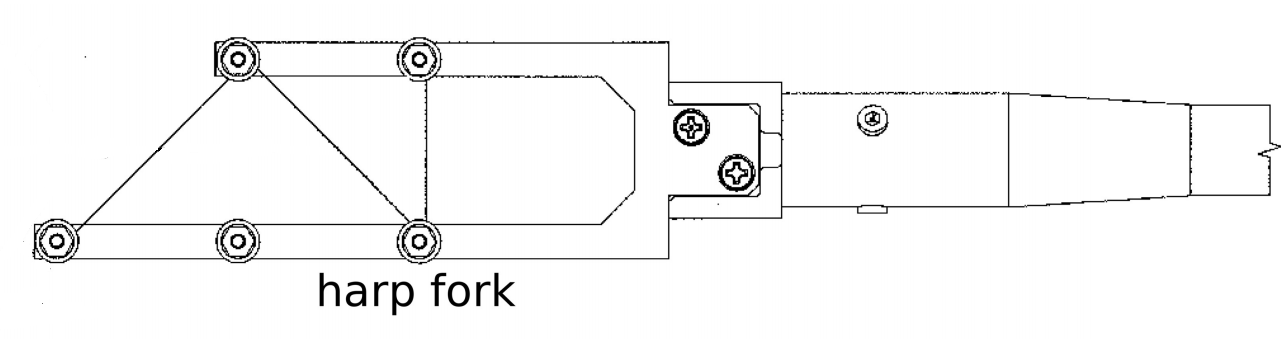
\includegraphics[width=14cm]{harp.png} 
		 	\end{figure}  	
	 
	 \paragraph{}The location of the wires on the harp frame and the position of the harp fork were used to calculate the absolute beam position. The BPM calibration coefficients were determine by using a bulls eye scan, figure \ref{bulls} shows an example of the five positions used to calculate the BPM calibration coefficients. The harp scan results are substituted into equation \ref{BPM_eq} for the X and Y positions. Using all five points and an $R^2$ regression technique, the coefficients can be determined with great accuracy. These highly accurate BPMs were crucial in reducing systematic error in the final results obtained from this experiment. 
	 \begin{equation}
	 \label{BPM_eq}
	 \begin{pmatrix}
	 X_{position}\\
	 Y_{position}
	 \end{pmatrix}
	=
		 \begin{pmatrix}
		 C(0,0) & C(0,1)\\
 		 C(0,0) & C(0,1)\\
		 \end{pmatrix}
		 *
		 	 \begin{pmatrix}
		 	 X_{BPM}\\
		 	 Y_{BPM}
		 	 \end{pmatrix}
		 	 +
		 	 \begin{pmatrix}
		 	 X_{offset}\\
		 	 Y_{offset}
		 	 \end{pmatrix}			 
	 	 \end{equation}
	
		\begin{figure}[H]
			\centering
			\caption{The X and Y position for a Bulls eye scan for BPM calibration. }
			\label{bulls}
			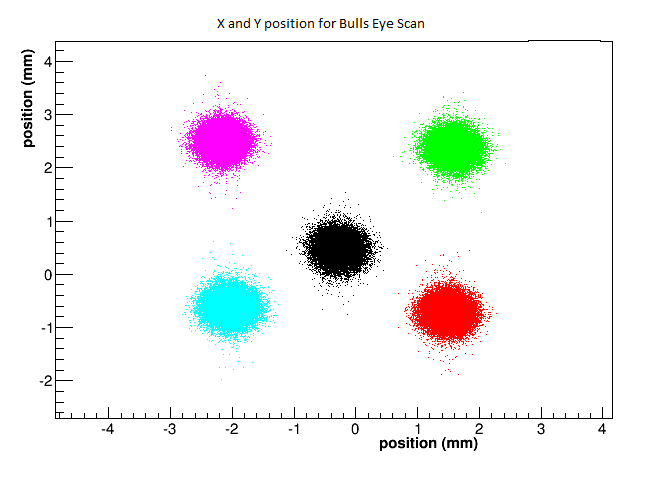
\includegraphics[width=10cm]{bulls.png} 
		\end{figure} 	
	